
\documentclass[11pt,a4paper,UTF8]{book}

\usepackage[T1]{fontenc}
\usepackage[utf8]{inputenc}
\usepackage{authblk}

\usepackage{ctex} %导入中文包
%\usepackage{ulem}
\usepackage{tocvsec2}

\usepackage{tabularx}
\usepackage{booktabs} 
\usepackage{multirow}
\usepackage{bbding}
\usepackage{float}
\usepackage{xspace}
\usepackage[none]{hyphenat}

\usepackage{graphicx}
\usepackage{subfigure}
\usepackage{pifont}

\usepackage{hyperref}  %制作pdf的目录
\usepackage{subfiles} %使用多文件方式进行

\usepackage{geometry} %设置页边距的包
\geometry{left=2.5cm,right=2cm,top=2.54cm,bottom=2.54cm} %设置书籍的页边距

\usepackage{url}
\hypersetup{hidelinks, %去红框
	colorlinks=true,
	allcolors=black,
	pdfstartview=Fit,
	breaklinks=true
}

% 调整itemlist中的行间距
\usepackage{enumitem}
\setenumerate[1]{itemsep=0pt,partopsep=0pt,parsep=\parskip,topsep=5pt}
\setitemize[1]{itemsep=0pt,partopsep=0pt,parsep=\parskip,topsep=5pt}
\setdescription{itemsep=0pt,partopsep=0pt,parsep=\parskip,topsep=5pt}

% 超链接样式设置
\usepackage{hyperref}
\hypersetup{
	colorlinks=true,
	linkcolor=blue,
	filecolor=blue,
	urlcolor=blue,
	citecolor=cyan,
}

\usepackage{indentfirst}

\usepackage{listings}
\usepackage[usenames,dvipsnames,svgnames, x11names]{xcolor}

\usepackage[most]{tcolorbox}

%展示代码
\definecolor{mygreen}{rgb}{0,0.6,0}
\definecolor{mygray}{rgb}{0.5,0.5,0.5}
\definecolor{mymauve}{rgb}{0.58,0,0.82}
\definecolor{keywordcolor}{rgb}{0.8,0.1,0.5}
\definecolor{webgreen}{rgb}{0,.5,0}
\definecolor{bgcolor}{rgb}{0.92,0.92,0.92}

%定义CMake
\lstdefinelanguage{CMake}
{morekeywords={
		cmake\_minimum\_required,
		project,
		add\_executable,
		add\_library,
		target\_link\_libraries,
		cmake\_parse\_arguments,
		cmake\_language,
		set, unset,
		option,
		string,
		list,
		math,
		message,
		if, elseif, else, endif,
		mark\_as\_advanced,
		foreach, endforeach,
		while, endwhile,
		add\_subdirectory, include, return, include\_gurad,
		function, endfunction,
		macro, endmacro,
		find\_package,
		cmake\_push\_check\_state,
		cmake\_pop\_check\_state,
		cmake\_reset\_check\_state,
		add\_test,
		set\_tests\_properties, 
		check\_c\_source\_runs,
		check\_cxx\_source\_runs,
		check\_fortran\_source\_runs,
		check\_source\_runs,
		check\_compiler\_flag,
		check\_c\_compiler\_flag,
		check\_cxx\_compiler\_flag,
		check\_fortran\_compiler\_flag,
		check\_symbol\_exists,
		check\_cxx\_symbol\_exists,
		check\_linker\_flag,
		cmake\_policy,
		set\_property,
		get\_property,
		define\_property,
		get\_cmake\_property,
		set\_cmake\_property,
		set\_target\_properties,
		get\_target\_property,
		set\_directory\_properties,
		get\_directory\_property,
		set\_source\_files\_properties,
		get\_source\_file\_property,
		set\_tests\_properties,
		get\_tests\_property,
		get\_test\_property,
		cmake\_print\_properties,
		cmake\_print\_variables,
		variable\_watch,
		include\_guard,
		target\_link\_options,
		target\_compile\_definitions,
		target\_compile\_options,
		include\_directories,
		add\_definitions,
		remove\_definitions,
		add\_compile\_definitions,
		add\_compile\_options,
		link\_libraries,
		link\_directories,
		add\_link\_options,
		target\_include\_directories,
		target\_compile\_features,
		add\_custom\_command,
		add\_custom\_target,
		execute\_process,
		cmake\_path,
		get\_filename\_component,
		file,
		configure\_file,
		generate\_export\_header,
		export,
		find\_file,
		find\_library,
		find\_package,
		find\_program,
		pkg\_check\_modules,
		pkg\_search\_module,
		pkg\_get\_variable,
		add\_test,
		enable\_testing,
		set\_tests\_properties,
		site\_name,
		ctest\_empty\_binary\_directory,
		ctest\_start,
		ctest\_configure,
		ctest\_submit,
		ctest\_build,
		ctest\_memcheck,
		ctest\_upload,
		ctest\_test,
		gtest\_add\_tests,
		gtest\_discover\_tests,
		install,
		write\_basic\_package\_version\_file,
		configure\_package\_config\_file,
		cpack\_add\_component,
		cpack\_add\_install\_type,
		cpack\_add\_component\_group,
		ExternalProject\_Add,
		ExternalProject\_Add\_StepDependencies,
		ExternalProject\_Get\_Property,
		ExternalProject\_Add\_Step,
		FetchContent\_Declare,
		FetchContent\_GetProperties,
		FetchContent\_Populate,
		source\_group,
		target\_precompile\_headers,
		qt5\_wrap\_cpp,
		qt5\_wrap\_ui,
		qt5\_add\_resources,
		qt5\_add\_big\_resources,
		qt5\_add\_binary\_resources,
		qt5\_add\_translation,
		qt5\_create\_translation,
		compile\_definitions,
		add\_llvm\_component\_library,
		add\_llvm\_tool,
		llvm\_multisource,
		llvm\_test\_data,
		doxygen\_add\_docs,
	}, %定义关键字
	sensitive=false, %是否大小写敏感
	morecomment=[l]{\#},
	morestring=[b]",
	morestring=[d]',
}

\lstdefinestyle{styleCXX}{
	language = C++,  
	backgroundcolor=\color{blue!3!white}, 
	%basicstyle = \footnotesize,  
	basicstyle      =   \zihao{-5}\ttfamily,
	numberstyle     =   \zihao{-5}\ttfamily,   
	%breakatwhitespace = false,    
	basewidth       =   0.5em,    
	breaklines = true,                 
	captionpos = b,                    
	commentstyle = \color{mygreen}\bfseries,
	%extendedchars = false,             
	frame =shadowbox, 
	framerule=0.5pt,
	%frameround = fttt,
	keepspaces=true,
	keywordstyle=\color{blue}\bfseries, % keyword style
	otherkeywords={string}, 
	numbers=left, 
	numbersep=5pt,
	numberstyle=\tiny\color{mygray},
	rulecolor=\color{black},         
	%showspaces=false,  
	%showstringspaces=false, 
	%showtabs=false,    
	%stepnumber=1,         
	stringstyle=\color{mymauve},        % string literal style
	tabsize=2,          
	columns         =   fixed,
	flexiblecolumns,                   
}


\lstdefinestyle{styleCMake}{
	language=CMake,
	backgroundcolor=\color{blue!3!white}, 
	basicstyle=\tt, 
	breakatwhitespace = false,
	breaklines = true,
	captionpos = b,
	commentstyle = \color{mygray}\bfseries, 
	extendedchars =false,             
	frame=shadowbox, 
	tabsize=2,
	framerule=0.5pt,
	keepspaces=true,
	keywordstyle=\color{blue}\bfseries, % keyword style
	otherkeywords={string}, 
	rulecolor=\color{black},
	showspaces=false,
	showstringspaces=false,
	showtabs=false,
	stepnumber=1,
	stringstyle=\color{purple},        % string literal style
}

\lstdefinestyle{stylePython}{
	language        =   Python, % 语言选Python
	backgroundcolor=\color{blue!3!white}, 
	basicstyle      =   \zihao{-5}\ttfamily,
	numberstyle     =   \zihao{-5}\ttfamily,
	keywordstyle    =   \color{blue},
	keywordstyle    =   [2] \color{teal},
	stringstyle     =   \color{magenta},
	commentstyle    =   \color{red}\ttfamily,
	frame = shadowbox, 
	breaklines      =   true,   % 自动换行,建议不要写太长的行
	columns         =   fixed,  % 如果不加这一句,字间距就不固定,很丑,必须加
	basewidth       =   0.5em,
	%basicstyle          =   \sffamily,          % 基本代码风格
	%keywordstyle        =   \bfseries,          % 关键字风格
	%commentstyle        =   \rmfamily\itshape,  % 注释的风格,斜体
	%stringstyle         =   \ttfamily,  % 字符串风格
	flexiblecolumns,                % 别问为什么,加上这个
	%numbers             =   left,   % 行号的位置在左边
	showspaces          =   false,  % 是否显示空格,显示了有点乱,所以不现实了
	numberstyle         =   \zihao{-5}\ttfamily,    % 行号的样式,小五号,tt等宽字体
	showstringspaces    =   false,
	captionpos          =   t,      % 这段代码的名字所呈现的位置,t指的是top上面
	frame               =   lrtb,   % 显示边框
	tabsize=2,  
}

\tcbset{
	commandshell/.style={
		listing only,
		colback=black!75!white,
		colupper=white,
		lowerbox=ignored,
		listing options={
			language={bash},
			basicstyle=\ttfamily,
			columns = fixed,
			flexiblecolumns
		}
}}

\usepackage{tikz}

% URL 正确换行
% https://liam.page/2017/05/17/help-the-url-command-from-hyperref-to-break-at-line-wrapping-point/
\makeatletter
\def\UrlAlphabet{%
	\do\a\do\b\do\c\do\d\do\e\do\f\do\g\do\h\do\i\do\j%
	\do\k\do\l\do\m\do\n\do\o\do\p\do\q\do\r\do\s\do\t%
	\do\u\do\v\do\w\do\x\do\y\do\z\do\A\do\B\do\C\do\D%
	\do\E\do\F\do\G\do\H\do\I\do\J\do\K\do\L\do\M\do\N%
	\do\O\do\P\do\Q\do\R\do\S\do\T\do\U\do\V\do\W\do\X%
	\do\Y\do\Z}
\def\UrlDigits{\do\1\do\2\do\3\do\4\do\5\do\6\do\7\do\8\do\9\do\0}
\g@addto@macro{\UrlBreaks}{\UrlOrds}
\g@addto@macro{\UrlBreaks}{\UrlAlphabet}
\g@addto@macro{\UrlBreaks}{\UrlDigits}
\makeatother

% enable subsubsubsection
% from https://tex.stackexchange.com/questions/274212/correct-hierarchy-levels-of-pdf-bookmarks-for-custom-section-subsubsubsection
\usepackage[depth=3]{bookmark}
\setcounter{secnumdepth}{3}
\setcounter{tocdepth}{4}
\hypersetup{bookmarksdepth=4}

\makeatletter

\newcommand{\toclevel@subsubsubsection}{4}
\newcounter{subsubsubsection}[subsubsection]

\renewcommand{\thesubsubsubsection}{\thesubsubsection.\arabic{subsubsubsection}}

\newcommand{\subsubsubsection}{\@startsection{subsubsubsection}{4}{\z@}%
	{-3.25ex\@plus -1ex \@minus -.2ex}%
	{1.5ex \@plus .2ex}%
	{\normalfont\normalsize\bf\bfseries}}

\newcommand*{\l@subsubsubsection}{\@dottedtocline{4}{11em}{5em}}  

\newcommand{\subsubsubsectionmark}[1]{}
\makeatother

\begin{document}
\begin{sloppypar} %latex中一行文字出现溢出问题的解决方法
	%\maketitle
	
	\begin{center}
		\thispagestyle{empty}
		%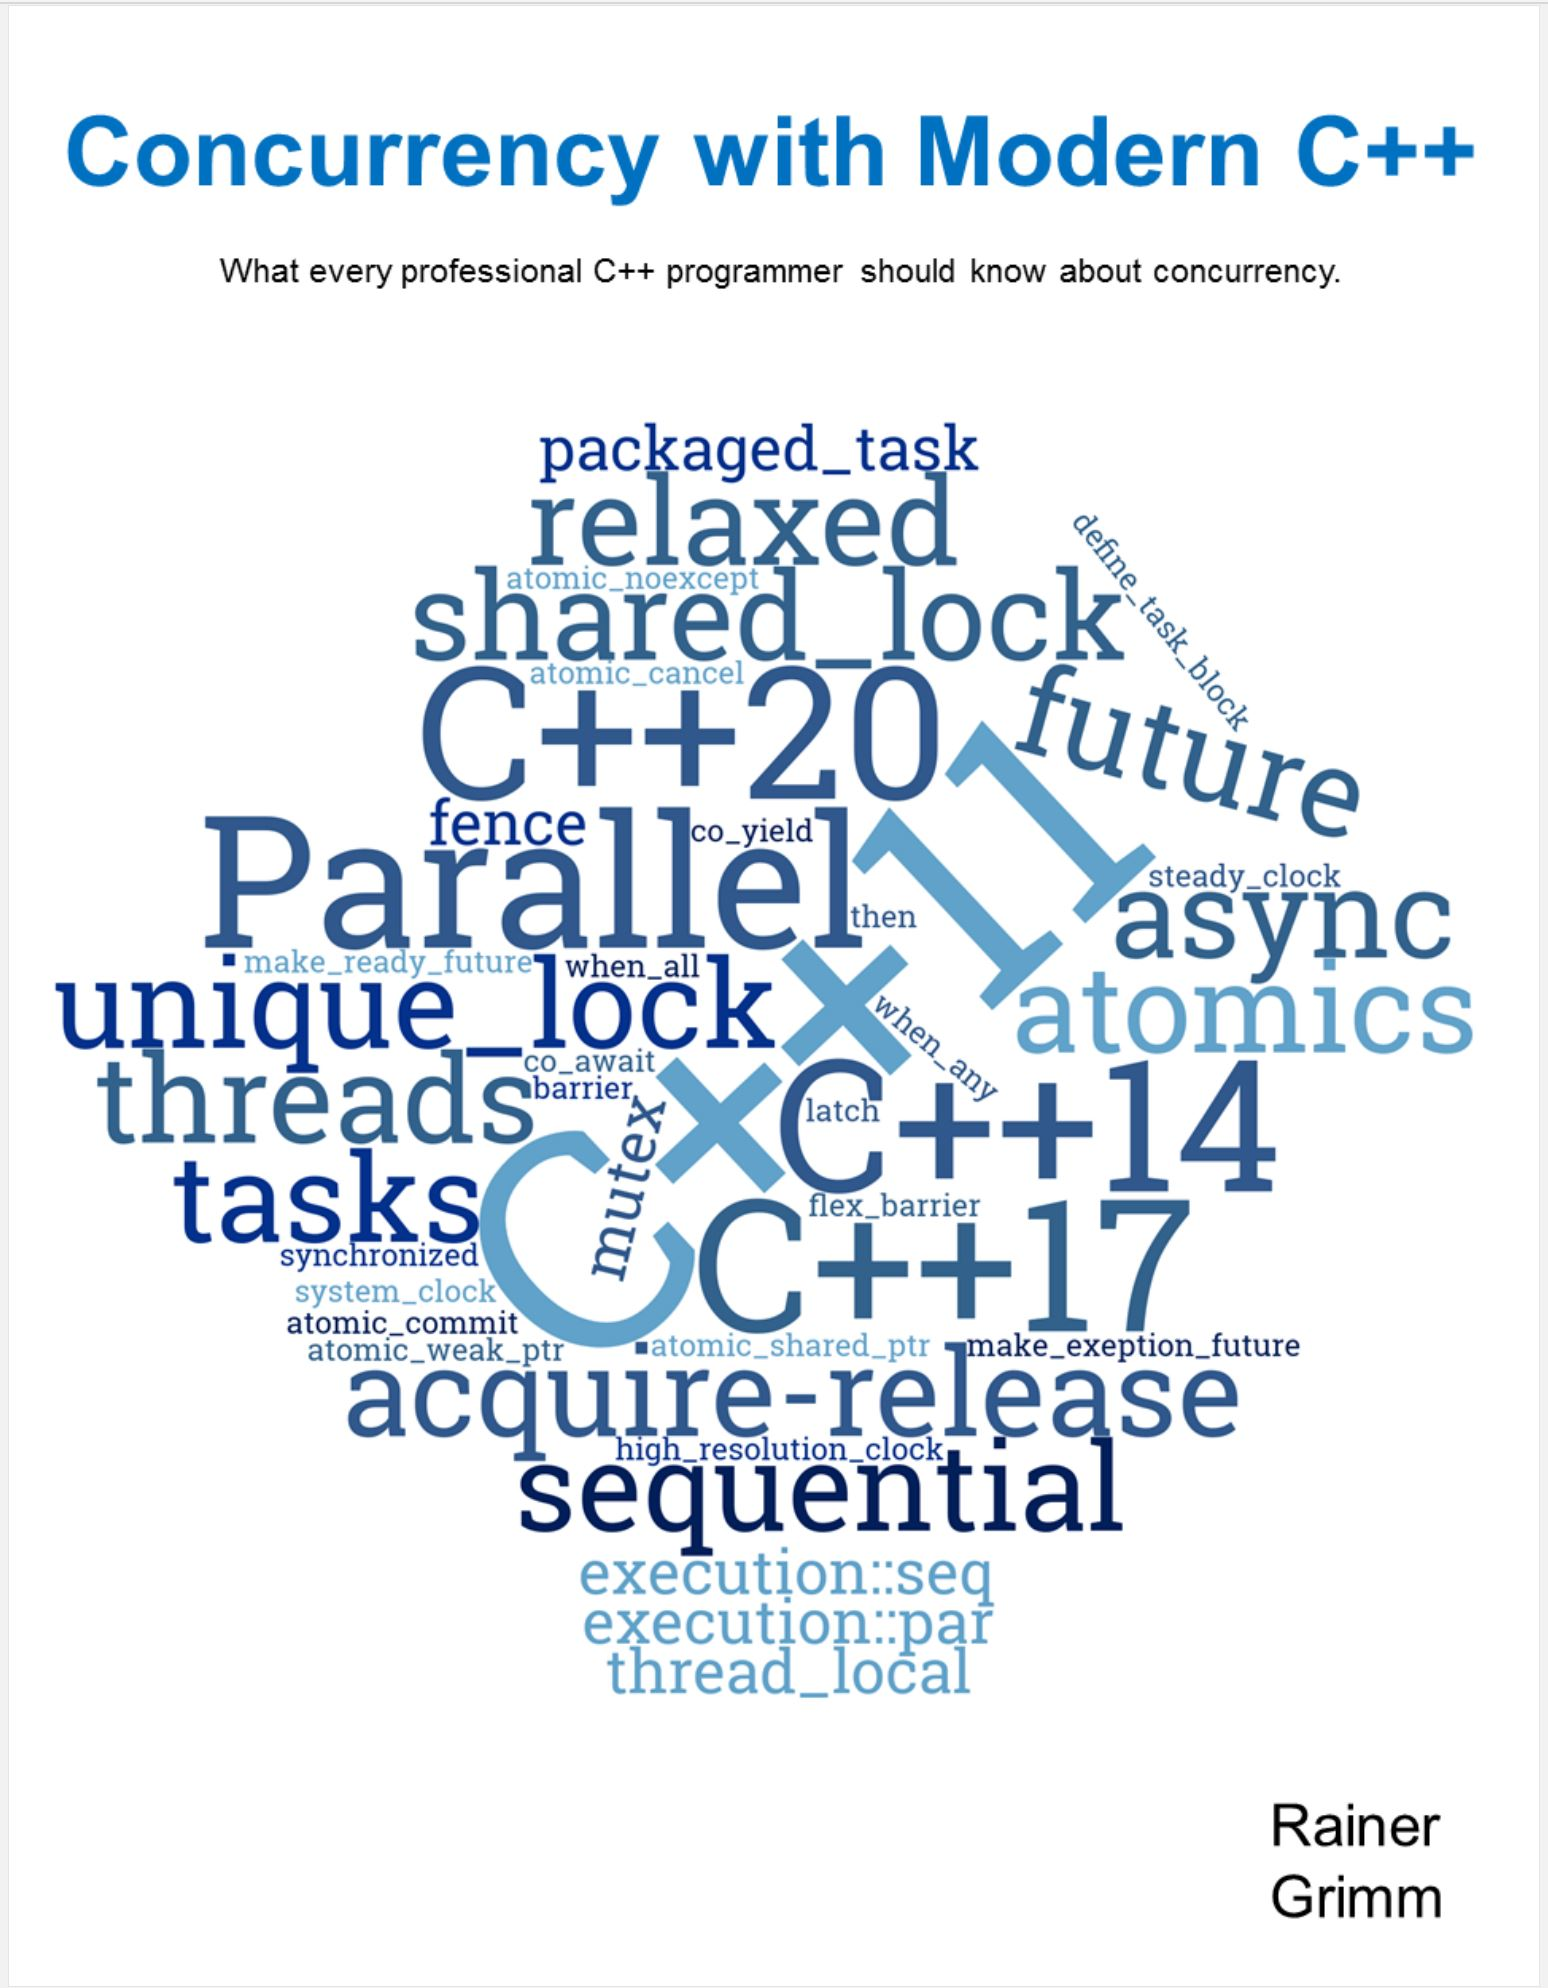
\includegraphics[width=\textwidth,height=\textheight,keepaspectratio]{cover.jpg}
		\begin{tikzpicture}[remember picture, overlay, inner sep=0pt]
			\node at (current page.center) 
			{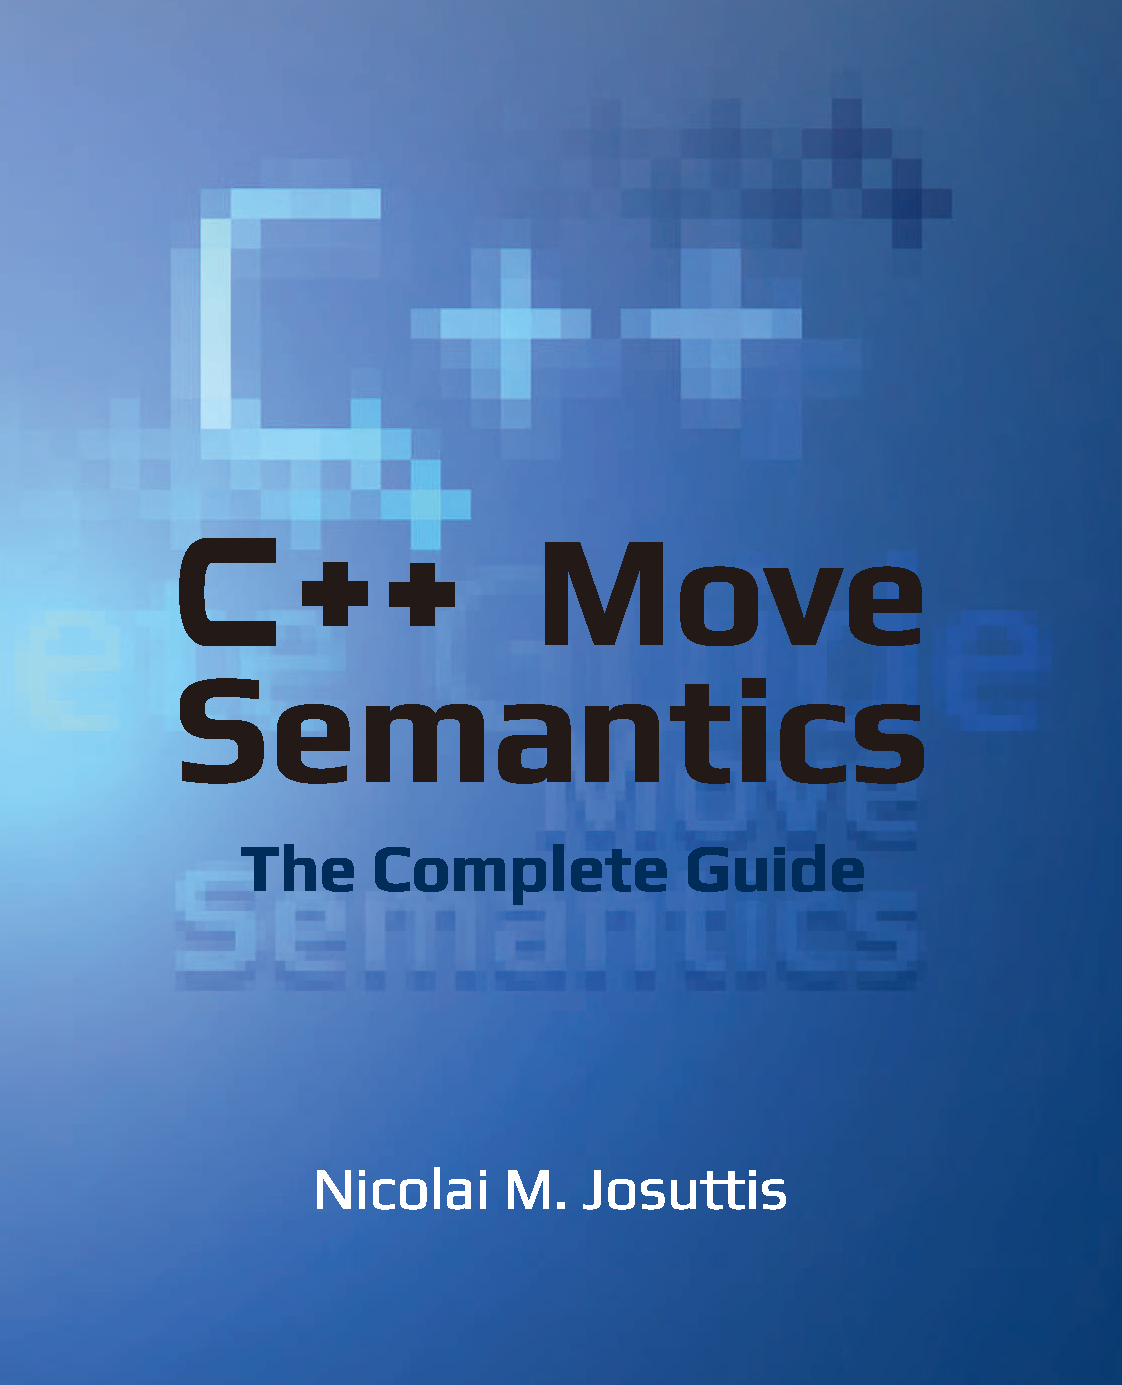
\includegraphics[width=\paperwidth, keepaspectratio=false]{cover.png}};
		\end{tikzpicture}
		\newpage
		\thispagestyle{empty}
		\huge
		\textbf{Software Architecture with C++} 
		\\[9pt]
		\normalsize
		Design modern systems using effective architecture concepts, design patterns, and techniques with C++20 \\ 
		(使用有效的架构概念,设计模式和C++20进行系统设计)
		\\[10pt]
		\normalsize 
		作者: Adrian Ostrowski,Piotr Gaczkowski
		\\[8pt]
		\normalsize
		译者;陈晓伟
	\end{center}
	
	\hspace*{\fill} \\ %插入空行
	\noindent\textbf{本书概述}
	
	\textit{通过理解诸如微服务、DevOps和使用现代C++标准和特性的本地云等架构,将业务需求应用到IT基础设施,并交付高质量的产品。}
	
	软件架构是指复杂应用的高级设计。就像语言一样,它也在不断发展,但在不牺牲可读性和可维护性的情况下,可以了解一些架构概念和模式,以及用高级语言编写高性能的应用。
	
	如果正在使用现代C++,本书会把相应的知识运用到实际工作中,设计分布式的、大规模的应用。首先,快速了解架构概念,包括已建立的模式和正在兴起的趋势,然后继续理解什么是软件架构,并开始研究其组件。
	
	接下来,在了解如何构建、打包、集成和部署组件之前,需要了解应用程序架构中涉及的设计概念和软件开发中的模式。最后一章,将探讨不同的架构质量,例如:可维护性、可重用性、可测试性、性能、可扩展性和安全性。最后,将概述分布式系统,如面向服务的架构、微服务和本地云,并了解如何在应用开发中应用。
	
	本书的最后,将使用现代C++和相关工具构建分布式服务,从而根据客户的需求交付解决方案。
	
	\hspace*{\fill} \\ %插入空行
	\noindent\textbf{关键特性}
	\begin{itemize}
		\item 用C++设计可扩展的大规模应用程序
		\item 基于云的持续集成和持续交付(CI/CD)中的软件架构解决方案
		\item 通过设计模式、语言特性和工具来实现架构的目标
	\end{itemize}
	
	\hspace*{\fill} \\ %插入空行
	\noindent\textbf{内容纲要}
	\begin{itemize}
		\item 理解如何应用软件架构的原则
		\item 应用设计模式和最佳实践来满足架构的目标
		\item 使用最新的C++特性编写优雅、安全、高效的代码
		\item 构建易于维护和部署的应用
		\item 探索不同架构的方法,并根据需求进行应用
		\item 使用容器简化开发和操作
		\item 了解软件设计和开发中常见问题的解决方法
	\end{itemize}
	
	\hspace*{\fill} \\ %插入空行
	\noindent\textbf{作者简介}
	
	\textbf{Adrian Ostrowski}是一个现代C++爱好者,对C++的开发和编写的高质量代码都很感兴趣。他在IT行业有超过十年的经验,特别是在C++方面有超过8年的经验,总是会与他人分享知识。其操刀的项目包括通过光纤网络进行并行计算,以及在商品交易所的交易系统上工作。目前,他是Intel和Habana机器学习框架的设计师之一。
	
	在业余时间里,他曾与Piotr一起推广乐队,并学会了驾驶滑翔机。目前,他喜欢骑自行车、参加音乐活动和浏览一些网络梗。
	
	\begin{center}
	\tt
	敬Agnieszka,感谢她的爱和支持
	
	敬Mateusz,我的良师益友
	
	敬我的父母,是你们激发了我的好奇心
	
	敬我的朋友们,感谢你们所做的一切
	\end{center}

	\textbf{Piotr Gaczkowski}在编程和实践DevOps方面有超过10年的经验。喜欢为问题构建简单的解决方案,组织文化活动,教授专业人士。Piotr热衷于将无聊的活动自动化,并利用自己的经验,通过开设课程、撰写有关个人成长和远程工作的文章来分享知识。
	
	他曾在IT行业从事全职工作和自由职业,但他真正热爱的是音乐。当技能不能在工作中发挥作用时,就会去在建立社区。
	
	\begin{center}
	\tt
	致Emilia,她在我写这本书的时候容非常包容我;
	
	我的父母鼓励我编程;为我加油鼓劲的智囊团成员;
	
	Hackerspace Trójmiasto,气氛组重要成员;
	
	IOD,提醒我要保持对写作的热爱;
	
	255,检验工作;
	
	以及所有和我一起走过这段旅程的朋友们。爱你们!
	\end{center}
	
	\thispagestyle{empty}
	\hspace*{\fill} \\ %插入空行
	\noindent\textbf{审评者介绍}
	
	\textbf{Andrey Gavrilin}是一名高级软件工程师,就职于提供财务管理云解决方案的国际公司。他拥有工程(工业自动化)硕士学位,曾在会计和人力资源、道路数据库、Web和Linux发行开发以及金融科技等不同领域工作。他的兴趣包括数学、电子、嵌入式系统、全栈网站开发、复古游戏和复古编程。
	
	
	\hspace*{\fill} \\ %插入空行
	\noindent\textbf{本书相关}
	\begin{itemize}
		\item Github翻译地址:\\\url{https://github.com/xiaoweiChen/Software-Architecture-with-Cpp}
	\end{itemize}
	\newpage
	
	%前言
	\pagestyle{empty}
	\subfile{content/preface.tex}
	
	\tableofcontents
	\newpage
	
	\setsecnumdepth{section}
	
	\color{white}
	\section*{\zihao{1}第一部分:软件架构的概念和组件}
	\pagecolor{mygray}
	\addcontentsline{toc}{section}{第一部分:软件架构的概念和组件}
	\textbf{\subfile{content/1/Section-1.tex}}
	\newpage
	\color{black}
	\pagecolor{white}
	
	\subsection*{\zihao{2} 第1章\hspace{0.5cm}软件架构的重要性和设计原则}
	\addcontentsline{toc}{subsection}{第1章\hspace{0.5cm}软件架构的重要性和设计原则}
	\subfile{content/1/chapter1/0.tex}
	
	\subsubsection*{\zihao{3} 1.1.\hspace{0.2cm}相关准备}
	\addcontentsline{toc}{subsubsection}{1.1.\hspace{0.2cm}相关准备}
	\subfile{content/1/chapter1/1.tex}
	
	\subsubsection*{\zihao{3} 1.2.\hspace{0.2cm}了解软件架构}
	\addcontentsline{toc}{subsubsection}{1.2.\hspace{0.2cm}了解软件架构}
	\subfile{content/1/chapter1/2.tex}
	
	\subsubsection*{\zihao{3} 1.3.\hspace{0.2cm}正确架构的重要性}
	\addcontentsline{toc}{subsubsection}{1.3.\hspace{0.2cm}正确架构的重要性}
	\subfile{content/1/chapter1/3.tex}
	
	\subsubsection*{\zihao{3} 1.4.\hspace{0.2cm}优秀架构的基础}
	\addcontentsline{toc}{subsubsection}{1.4.\hspace{0.2cm}优秀架构的基础}
	\subfile{content/1/chapter1/4.tex}
	
	\subsubsection*{\zihao{3} 1.5.\hspace{0.2cm}使用敏捷原则开发软件架构}
	\addcontentsline{toc}{subsubsection}{1.5.\hspace{0.2cm}使用敏捷原则开发软件架构}
	\subfile{content/1/chapter1/5.tex}
	
	\subsubsection*{\zihao{3} 1.6.\hspace{0.2cm}C++的哲学}
	\addcontentsline{toc}{subsubsection}{1.6.\hspace{0.2cm}C++的哲学}
	\subfile{content/1/chapter1/6.tex}
	
	\subsubsection*{\zihao{3} 1.7.\hspace{0.2cm}SOLID和DRY原则}
	\addcontentsline{toc}{subsubsection}{1.7.\hspace{0.2cm}SOLID和DRY原则}
	\subfile{content/1/chapter1/7.tex}
	
	\subsubsection*{\zihao{3} 1.8.\hspace{0.2cm}耦合和内聚}
	\addcontentsline{toc}{subsubsection}{1.8.\hspace{0.2cm}耦合和内聚}
	\subfile{content/1/chapter1/8.tex}
	
	\subsubsection*{\zihao{3} 1.9.\hspace{0.2cm}总结}
	\addcontentsline{toc}{subsubsection}{1.9.\hspace{0.2cm}总结}
	\subfile{content/1/chapter1/9.tex}
	
	\subsubsection*{\zihao{3} 1.10.\hspace{0.2cm}练习题}
	\addcontentsline{toc}{subsubsection}{1.10.\hspace{0.2cm}练习题}
	\subfile{content/1/chapter1/10.tex}
	
	\subsubsection*{\zihao{3} 1.11.\hspace{0.2cm}扩展阅读}
	\addcontentsline{toc}{subsubsection}{1.11.\hspace{0.2cm}扩展阅读}
	\subfile{content/1/chapter1/11.tex}
	\newpage
	
	\subsection*{\zihao{2} 第2章\hspace{0.5cm}架构风格}
	\addcontentsline{toc}{subsection}{第2章\hspace{0.5cm}架构风格}
	\subfile{content/1/chapter2/0.tex}
	
	\subsubsection*{\zihao{3} 2.1.\hspace{0.2cm}相关准备}
	\addcontentsline{toc}{subsubsection}{2.1.\hspace{0.2cm}相关准备}
	\subfile{content/1/chapter2/1.tex}
	
	\subsubsection*{\zihao{3} 2.2.\hspace{0.2cm}选择有状态方法和无状态方法}
	\addcontentsline{toc}{subsubsection}{2.2.\hspace{0.2cm}选择有状态方法和无状态方法}
	\subfile{content/1/chapter2/2.tex}
	
	\subsubsection*{\zihao{3} 2.3.\hspace{0.2cm}理解大应用——避免使用的原因,以及识别异常}
	\addcontentsline{toc}{subsubsection}{2.3.\hspace{0.2cm}理解大应用——避免使用的原因,以及识别异常}
	\subfile{content/1/chapter2/3.tex}
	
	\subsubsection*{\zihao{3} 2.4.\hspace{0.2cm}理解服务和微服务}
	\addcontentsline{toc}{subsubsection}{2.4.\hspace{0.2cm}理解服务和微服务}
	\subfile{content/1/chapter2/4.tex}
	
	\subsubsection*{\zihao{3} 2.5.\hspace{0.2cm}探索基于事件的架构}
	\addcontentsline{toc}{subsubsection}{2.5.\hspace{0.2cm}探索基于事件的架构}
	\subfile{content/1/chapter2/5.tex}
	
	\subsubsection*{\zihao{3} 2.6.\hspace{0.2cm}探索分层架构}
	\addcontentsline{toc}{subsubsection}{2.6.\hspace{0.2cm}探索分层架构}
	\subfile{content/1/chapter2/6.tex}
	
	\subsubsection*{\zihao{3} 2.7.\hspace{0.2cm}了解模块化架构}
	\addcontentsline{toc}{subsubsection}{2.7.\hspace{0.2cm}了解模块化架构}
	\subfile{content/1/chapter2/7.tex}
	
	\subsubsection*{\zihao{3} 2.8.\hspace{0.2cm}总结}
	\addcontentsline{toc}{subsubsection}{2.8.\hspace{0.2cm}总结}
	\subfile{content/1/chapter2/8.tex}
	
	\subsubsection*{\zihao{3} 2.9.\hspace{0.2cm}练习题}
	\addcontentsline{toc}{subsubsection}{2.9.\hspace{0.2cm}练习题}
	\subfile{content/1/chapter2/9.tex}
	
	\subsubsection*{\zihao{3} 2.10.\hspace{0.2cm}扩展阅读}
	\addcontentsline{toc}{subsubsection}{2.10.\hspace{0.2cm}扩展阅读}
	\subfile{content/1/chapter2/10.tex}
	\newpage
	
	\subsection*{\zihao{2} 第3章\hspace{0.5cm}功能和非功能需求}
	\addcontentsline{toc}{subsection}{第3章\hspace{0.5cm}功能和非功能需求}
	\subfile{content/1/chapter3/0.tex}
	
	\subsubsection*{\zihao{3} 3.1.\hspace{0.2cm}相关准备}
	\addcontentsline{toc}{subsubsection}{3.1.\hspace{0.2cm}相关准备}
	\subfile{content/1/chapter3/1.tex}
	
	\subsubsection*{\zihao{3} 3.2.\hspace{0.2cm}需求类型}
	\addcontentsline{toc}{subsubsection}{3.2.\hspace{0.2cm}需求类型}
	\subfile{content/1/chapter3/2.tex}
	
	\subsubsection*{\zihao{3} 3.3.\hspace{0.2cm}认识架构的重要需求}
	\addcontentsline{toc}{subsubsection}{3.3.\hspace{0.2cm}认识架构的重要需求}
	\subfile{content/1/chapter3/3.tex}
	
	\subsubsection*{\zihao{3} 3.4.\hspace{0.2cm}收集需求}
	\addcontentsline{toc}{subsubsection}{3.4.\hspace{0.2cm}收集需求}
	\subfile{content/1/chapter3/4.tex}
	
	\subsubsection*{\zihao{3} 3.5.\hspace{0.2cm}文档化需求}
	\addcontentsline{toc}{subsubsection}{3.5.\hspace{0.2cm}文档化需求}
	\subfile{content/1/chapter3/5.tex}
	
	\subsubsection*{\zihao{3} 3.6.\hspace{0.2cm}文档化架构}
	\addcontentsline{toc}{subsubsection}{3.6.\hspace{0.2cm}文档化架构}
	\subfile{content/1/chapter3/6.tex}
	
	\subsubsection*{\zihao{3} 3.7.\hspace{0.2cm}选择合适的视图进行记录}
	\addcontentsline{toc}{subsubsection}{3.7.\hspace{0.2cm}选择合适的视图进行记录}
	\subfile{content/1/chapter3/7.tex}
	
	\subsubsection*{\zihao{3} 3.8.\hspace{0.2cm}生成文档}
	\addcontentsline{toc}{subsubsection}{3.8.\hspace{0.2cm}生成文档}
	\subfile{content/1/chapter3/8.tex}
	
	\subsubsection*{\zihao{3} 3.9.\hspace{0.2cm}总结}
	\addcontentsline{toc}{subsubsection}{3.9.\hspace{0.2cm}总结}
	\subfile{content/1/chapter3/9.tex}
	
	\subsubsection*{\zihao{3} 3.10.\hspace{0.2cm}练习题}
	\addcontentsline{toc}{subsubsection}{3.10.\hspace{0.2cm}练习题}
	\subfile{content/1/chapter3/10.tex}
	
	\subsubsection*{\zihao{3} 3.11.\hspace{0.2cm}扩展阅读}
	\addcontentsline{toc}{subsubsection}{3.11.\hspace{0.2cm}扩展阅读}
	\subfile{content/1/chapter3/11.tex}
	\newpage
	
	\color{white}
	\section*{\zihao{1}第二部分:C++软件的设计与开发}
	\pagecolor{mygray}
	\addcontentsline{toc}{section}{第二部分:C++软件的设计与开发}
	\textbf{\subfile{content/2/Section-2.tex}}
	\newpage
	\color{black}
	\pagecolor{white}
	
	\subsection*{\zihao{2} 第4章\hspace{0.5cm}架构与系统设计}
	\addcontentsline{toc}{subsection}{第4章\hspace{0.5cm}架构与系统设计}
	\subfile{content/2/chapter4/0.tex}
	
	\subsubsection*{\zihao{3} 4.1.\hspace{0.2cm}相关准备}
	\addcontentsline{toc}{subsubsection}{4.1.\hspace{0.2cm}相关准备}
	\subfile{content/2/chapter4/1.tex}
	
	\subsubsection*{\zihao{3} 4.2.\hspace{0.2cm}分布式系统的特性}
	\addcontentsline{toc}{subsubsection}{4.2.\hspace{0.2cm}分布式系统的特性}
	\subfile{content/2/chapter4/2.tex}
	
	\subsubsection*{\zihao{3} 4.3.\hspace{0.2cm}使系统具有容错性和可用性}
	\addcontentsline{toc}{subsubsection}{4.3.\hspace{0.2cm}使系统具有容错性和可用性}
	\subfile{content/2/chapter4/3.tex}
	
	\subsubsection*{\zihao{3} 4.4.\hspace{0.2cm}集成系统}
	\addcontentsline{toc}{subsubsection}{4.4.\hspace{0.2cm}集成系统}
	\subfile{content/2/chapter4/4.tex}
	
	\subsubsection*{\zihao{3} 4.5.\hspace{0.2cm}分级性能}
	\addcontentsline{toc}{subsubsection}{4.5.\hspace{0.2cm}分级性能}
	\subfile{content/2/chapter4/5.tex}
	
	\subsubsection*{\zihao{3} 4.6.\hspace{0.2cm}部署系统}
	\addcontentsline{toc}{subsubsection}{4.6.\hspace{0.2cm}部署系统}
	\subfile{content/2/chapter4/6.tex}
	
	\subsubsection*{\zihao{3} 4.7.\hspace{0.2cm}管理API}
	\addcontentsline{toc}{subsubsection}{4.7.\hspace{0.2cm}管理API}
	\subfile{content/2/chapter4/7.tex}
	
	\subsubsection*{\zihao{3} 4.8.\hspace{0.2cm}总结}
	\addcontentsline{toc}{subsubsection}{4.8.\hspace{0.2cm}总结}
	\subfile{content/2/chapter4/8.tex}
	
	\subsubsection*{\zihao{3} 4.9.\hspace{0.2cm}练习题}
	\addcontentsline{toc}{subsubsection}{4.9.\hspace{0.2cm}练习题}
	\subfile{content/2/chapter4/9.tex}
	
	\subsubsection*{\zihao{3} 4.10.\hspace{0.2cm}扩展阅读}
	\addcontentsline{toc}{subsubsection}{4.10.\hspace{0.2cm}扩展阅读}
	\subfile{content/2/chapter4/10.tex}
	\newpage
	
	\subsection*{\zihao{2} 第5章\hspace{0.5cm}C++特性}
	\addcontentsline{toc}{subsection}{第5章\hspace{0.5cm}C++特性}
	\subfile{content/2/chapter5/0.tex}
	
	\subsubsection*{\zihao{3} 5.1.\hspace{0.2cm}相关准备}
	\addcontentsline{toc}{subsubsection}{5.1.\hspace{0.2cm}相关准备}
	\subfile{content/2/chapter5/1.tex}
	
	\subsubsection*{\zihao{3} 5.2.\hspace{0.2cm}设计优秀的API}
	\addcontentsline{toc}{subsubsection}{5.2.\hspace{0.2cm}设计优秀的API}
	\subfile{content/2/chapter5/2.tex}
	
	\subsubsection*{\zihao{3} 5.3.\hspace{0.2cm}编写声明性代码}
	\addcontentsline{toc}{subsubsection}{5.3.\hspace{0.2cm}编写声明性代码}
	\subfile{content/2/chapter5/3.tex}
	
	\subsubsection*{\zihao{3} 5.4.\hspace{0.2cm}编译时计算}
	\addcontentsline{toc}{subsubsection}{5.4.\hspace{0.2cm}编译时计算}
	\subfile{content/2/chapter5/4.tex}
	
	\subsubsection*{\zihao{3} 5.5.\hspace{0.2cm}安全类型}
	\addcontentsline{toc}{subsubsection}{5.5.\hspace{0.2cm}安全类型}
	\subfile{content/2/chapter5/5.tex}
	
	\subsubsection*{\zihao{3} 5.6.\hspace{0.2cm}编写模块化C++}
	\addcontentsline{toc}{subsubsection}{5.6.\hspace{0.2cm}编写模块化C++}
	\subfile{content/2/chapter5/6.tex}
	
	\subsubsection*{\zihao{3} 5.7.\hspace{0.2cm}总结}
	\addcontentsline{toc}{subsubsection}{5.7.\hspace{0.2cm}总结}
	\subfile{content/2/chapter5/7.tex}
	
	\subsubsection*{\zihao{3} 5.8.\hspace{0.2cm}练习题}
	\addcontentsline{toc}{subsubsection}{5.8.\hspace{0.2cm}练习题}
	\subfile{content/2/chapter5/8.tex}
	
	\subsubsection*{\zihao{3} 5.9.\hspace{0.2cm}扩展阅读}
	\addcontentsline{toc}{subsubsection}{5.9.\hspace{0.2cm}扩展阅读}
	\subfile{content/2/chapter5/9.tex}
	\newpage
	
	\subsection*{\zihao{2} 第6章\hspace{0.5cm}设计模式和C++}
	\addcontentsline{toc}{subsection}{第6章\hspace{0.5cm}设计模式和C++}
	\subfile{content/2/chapter6/0.tex}
	
	\subsubsection*{\zihao{3} 6.1.\hspace{0.2cm}相关准备}
	\addcontentsline{toc}{subsubsection}{6.1.\hspace{0.2cm}相关准备}
	\subfile{content/2/chapter6/1.tex}
	
	\subsubsection*{\zihao{3} 6.2.\hspace{0.2cm}C++的惯用法}
	\addcontentsline{toc}{subsubsection}{6.2.\hspace{0.2cm}C++的惯用法}
	\subfile{content/2/chapter6/2.tex}
	
	\subsubsection*{\zihao{3} 6.3.\hspace{0.2cm}模板递归模式}
	\addcontentsline{toc}{subsubsection}{6.3.\hspace{0.2cm}模板递归模式}
	\subfile{content/2/chapter6/3.tex}
	
	\subsubsection*{\zihao{3} 6.4.\hspace{0.2cm}创建对象}
	\addcontentsline{toc}{subsubsection}{6.4.\hspace{0.2cm}创建对象}
	\subfile{content/2/chapter6/4.tex}
	
	\subsubsection*{\zihao{3} 6.5.\hspace{0.2cm}C++中跟踪状态和访问对象}
	\addcontentsline{toc}{subsubsection}{6.5.\hspace{0.2cm}C++中跟踪状态和访问对象}
	\subfile{content/2/chapter6/5.tex}
	
	\subsubsection*{\zihao{3} 6.6.\hspace{0.2cm}高效地处理内存}
	\addcontentsline{toc}{subsubsection}{6.6.\hspace{0.2cm}高效地处理内存}
	\subfile{content/2/chapter6/6.tex}
	
	\subsubsection*{\zihao{3} 6.7\hspace{0.2cm}总结}
	\addcontentsline{toc}{subsubsection}{6.7.\hspace{0.2cm}总结}
	\subfile{content/2/chapter6/7.tex}
	
	\subsubsection*{\zihao{3} 6.8.\hspace{0.2cm}练习题}
	\addcontentsline{toc}{subsubsection}{6.8.\hspace{0.2cm}练习题}
	\subfile{content/2/chapter6/8.tex}
	
	\subsubsection*{\zihao{3} 6.9.\hspace{0.2cm}扩展阅读}
	\addcontentsline{toc}{subsubsection}{6.9.\hspace{0.2cm}扩展阅读}
	\subfile{content/2/chapter6/9.tex}
	\newpage
	
	\subsection*{\zihao{2} 第7章\hspace{0.5cm}构建和打包}
	\addcontentsline{toc}{subsection}{第7章\hspace{0.5cm}构建和打包}
	\subfile{content/2/chapter7/0.tex}
	
	\subsubsection*{\zihao{3} 7.1.\hspace{0.2cm}相关准备}
	\addcontentsline{toc}{subsubsection}{7.1.\hspace{0.2cm}相关准备}
	\subfile{content/2/chapter7/1.tex}
	
	\subsubsection*{\zihao{3} 7.2.\hspace{0.2cm}充分利用编译器}
	\addcontentsline{toc}{subsubsection}{7.2.\hspace{0.2cm}充分利用编译器}
	\subfile{content/2/chapter7/2.tex}
	
	\subsubsection*{\zihao{3} 7.3.\hspace{0.2cm}抽象构建过程}
	\addcontentsline{toc}{subsubsection}{7.3.\hspace{0.2cm}抽象构建过程}
	\subfile{content/2/chapter7/3.tex}
	
	\subsubsection*{\zihao{3} 7.4.\hspace{0.2cm}使用外部模块}
	\addcontentsline{toc}{subsubsection}{7.4.\hspace{0.2cm}使用外部模块}
	\subfile{content/2/chapter7/4.tex}
	
	\subsubsection*{\zihao{3} 7.5.\hspace{0.2cm}重用代码质量}
	\addcontentsline{toc}{subsubsection}{7.5.\hspace{0.2cm}重用代码质量}
	\subfile{content/2/chapter7/5.tex}
	
	\subsubsection*{\zihao{3} 7.6.\hspace{0.2cm}使用Conan进行打包}
	\addcontentsline{toc}{subsubsection}{7.6.\hspace{0.2cm}使用Conan进行打包}
	\subfile{content/2/chapter7/6.tex}
	
	\subsubsection*{\zihao{3} 7.7.\hspace{0.2cm}总结}
	\addcontentsline{toc}{subsubsection}{7.7.\hspace{0.2cm}总结}
	\subfile{content/2/chapter7/7.tex}
	
	\subsubsection*{\zihao{3} 7.8.\hspace{0.2cm}练习题}
	\addcontentsline{toc}{subsubsection}{7.8.\hspace{0.2cm}练习题}
	\subfile{content/2/chapter7/8.tex}
	
	\subsubsection*{\zihao{3} 7.9.\hspace{0.2cm}扩展阅读}
	\addcontentsline{toc}{subsubsection}{7.9.\hspace{0.2cm}扩展阅读}
	\subfile{content/2/chapter7/9.tex}
	\newpage
	
	\color{white}
	\section*{\zihao{1}第三部分:体系架构的质量}
	\pagecolor{mygray}
	\addcontentsline{toc}{section}{第三部分:体系架构的质量}
	\textbf{\subfile{content/3/Section-3.tex}}
	\newpage
	\color{black}
	\pagecolor{white}
	
	\subsection*{\zihao{2} 第8章\hspace{0.5cm}编写可测试的代码}
	\addcontentsline{toc}{subsection}{第8章\hspace{0.5cm}编写可测试的代码}
	\subfile{content/3/chapter8/0.tex}
	
	\subsubsection*{\zihao{3} 8.1.\hspace{0.2cm}相关准备}
	\addcontentsline{toc}{subsubsection}{8.1.\hspace{0.2cm}相关准备}
	\subfile{content/3/chapter8/1.tex}
	
	\subsubsection*{\zihao{3} 8.2.\hspace{0.2cm}为什么要写测试代码?}
	\addcontentsline{toc}{subsubsection}{8.2.\hspace{0.2cm}为什么要写测试代码?}
	\subfile{content/3/chapter8/2.tex}
	
	\subsubsection*{\zihao{3} 8.3.\hspace{0.2cm}测试框架}
	\addcontentsline{toc}{subsubsection}{8.3.\hspace{0.2cm}测试框架}
	\subfile{content/3/chapter8/3.tex}
	
	\subsubsection*{\zihao{3} 8.4.\hspace{0.2cm}测试中的mock和fake}
	\addcontentsline{toc}{subsubsection}{8.4.\hspace{0.2cm}测试中的mock和fake}
	\subfile{content/3/chapter8/4.tex}
	
	\subsubsection*{\zihao{3} 8.5.\hspace{0.2cm}测试驱动的类型设计}
	\addcontentsline{toc}{subsubsection}{8.5.\hspace{0.2cm}测试驱动的类型设计}
	\subfile{content/3/chapter8/5.tex}
	
	\subsubsection*{\zihao{3} 8.6.\hspace{0.2cm}在持续集成/持续部署上进行自动化测试}
	\addcontentsline{toc}{subsubsection}{8.6.\hspace{0.2cm}在持续集成/持续部署上进行自动化测试}
	\subfile{content/3/chapter8/6.tex}
	
	\subsubsection*{\zihao{3} 8.7.\hspace{0.2cm}总结}
	\addcontentsline{toc}{subsubsection}{8.7.\hspace{0.2cm}总结}
	\subfile{content/3/chapter8/7.tex}
	
	\subsubsection*{\zihao{3} 8.8.\hspace{0.2cm}练习题}
	\addcontentsline{toc}{subsubsection}{8.8.\hspace{0.2cm}练习题}
	\subfile{content/3/chapter8/8.tex}
	
	\subsubsection*{\zihao{3} 8.9.\hspace{0.2cm}扩展阅读}
	\addcontentsline{toc}{subsubsection}{8.9.\hspace{0.2cm}扩展阅读}
	\subfile{content/3/chapter8/9.tex}
	\newpage
	
	\subsection*{\zihao{2} 第9章\hspace{0.5cm}持续集成和持续部署}
	\addcontentsline{toc}{subsection}{第9章\hspace{0.5cm}持续集成和持续部署}
	\subfile{content/3/chapter9/0.tex}
	
	\subsubsection*{\zihao{3} 9.1.\hspace{0.2cm}相关准备}
	\addcontentsline{toc}{subsubsection}{9.1.\hspace{0.2cm}相关准备}
	\subfile{content/3/chapter9/1.tex}
	
	\subsubsection*{\zihao{3} 9.2.\hspace{0.2cm}了解CI}
	\addcontentsline{toc}{subsubsection}{9.2.\hspace{0.2cm}了解CI}
	\subfile{content/3/chapter9/2.tex}
	
	\subsubsection*{\zihao{3} 9.3.\hspace{0.2cm}检查代码更改}
	\addcontentsline{toc}{subsubsection}{9.3.\hspace{0.2cm}检查代码更改}	
	\subfile{content/3/chapter9/3.tex}
	
	\subsubsection*{\zihao{3} 9.4.\hspace{0.2cm}探索测试驱动的自动化}
	\addcontentsline{toc}{subsubsection}{9.4.\hspace{0.2cm}探索测试驱动的自动化}
	\subfile{content/3/chapter9/4.tex}
	
	\subsubsection*{\zihao{3} 9.5.\hspace{0.2cm}管理部署代码}
	\addcontentsline{toc}{subsubsection}{9.5.\hspace{0.2cm}管理部署代码}
	\subfile{content/3/chapter9/5.tex}
	
	\subsubsection*{\zihao{3} 9.6.\hspace{0.2cm}构建部署代码}
	\addcontentsline{toc}{subsubsection}{9.6.\hspace{0.2cm}构建部署代码}
	\subfile{content/3/chapter9/6.tex}
	
	\subsubsection*{\zihao{3} 9.7.\hspace{0.2cm}建立CD流水线}
	\addcontentsline{toc}{subsubsection}{9.7.\hspace{0.2cm}建立CD流水线}
	\subfile{content/3/chapter9/7.tex}
	
	\subsubsection*{\zihao{3} 9.8.\hspace{0.2cm}不可变的基础设施}
	\addcontentsline{toc}{subsubsection}{9.8.\hspace{0.2cm}不可变的基础设施}
	\subfile{content/3/chapter9/8.tex}
	
	\subsubsection*{\zihao{3} 9.9.\hspace{0.2cm}总结}
	\addcontentsline{toc}{subsubsection}{9.9.\hspace{0.2cm}总结}
	\subfile{content/3/chapter9/9.tex}
	
	\subsubsection*{\zihao{3} 9.10.\hspace{0.2cm}练习题}
	\addcontentsline{toc}{subsubsection}{9.10.\hspace{0.2cm}练习题}
	\subfile{content/3/chapter9/10.tex}
	
	\subsubsection*{\zihao{3} 9.11.\hspace{0.2cm}扩展阅读}
	\addcontentsline{toc}{subsubsection}{9.11.\hspace{0.2cm}扩展阅读}
	\subfile{content/3/chapter9/11.tex}
	\newpage
	
	\subsection*{\zihao{2} 第10章\hspace{0.5cm}代码和部署的安全性}
	\addcontentsline{toc}{subsection}{第10章\hspace{0.5cm}代码和部署的安全性}
	\subfile{content/3/chapter10/0.tex}
	
	\subsubsection*{\zihao{3} 10.1.\hspace{0.2cm}相关准备}
	\addcontentsline{toc}{subsubsection}{10.1.\hspace{0.2cm}相关准备}
	\subfile{content/3/chapter10/1.tex}
	
	\subsubsection*{\zihao{3} 10.2.\hspace{0.2cm}检查代码安全性}
	\addcontentsline{toc}{subsubsection}{10.2.\hspace{0.2cm}检查代码安全性}
	\subfile{content/3/chapter10/2.tex}
	
	\subsubsection*{\zihao{3} 10.3.\hspace{0.2cm}检查依赖关系是否安全}
	\addcontentsline{toc}{subsubsection}{10.3.\hspace{0.2cm}检查依赖关系是否安全}
	\subfile{content/3/chapter10/3.tex}
	
	\subsubsection*{\zihao{3} 10.4.\hspace{0.2cm}加固代码}
	\addcontentsline{toc}{subsubsection}{10.4.\hspace{0.2cm}加固代码}
	\subfile{content/3/chapter10/4.tex}
	
	\subsubsection*{\zihao{3} 10.5.\hspace{0.2cm}强化环境}
	\addcontentsline{toc}{subsubsection}{10.5.\hspace{0.2cm}强化环境}
	\subfile{content/3/chapter10/5.tex}
	
	\subsubsection*{\zihao{3} 10.6.\hspace{0.2cm}总结}
	\addcontentsline{toc}{subsubsection}{10.6.\hspace{0.2cm}总结}
	\subfile{content/3/chapter10/6.tex}
	
	\subsubsection*{\zihao{3} 10.7.\hspace{0.2cm}练习题}
	\addcontentsline{toc}{subsubsection}{10.7.\hspace{0.2cm}练习题}
	\subfile{content/3/chapter10/7.tex}
	
	\subsubsection*{\zihao{3} 10.8.\hspace{0.2cm}扩展阅读}
	\addcontentsline{toc}{subsubsection}{10.8.\hspace{0.2cm}扩展阅读}
	\subfile{content/3/chapter10/8.tex}
	\newpage
	
	\subsection*{\zihao{2} 第11章\hspace{0.5cm}性能}
	\addcontentsline{toc}{subsection}{第11章\hspace{0.5cm}性能}
	\subfile{content/3/chapter11/0.tex}
	
	\subsubsection*{\zihao{3} 11.1.\hspace{0.2cm}相关准备}
	\addcontentsline{toc}{subsubsection}{11.1.\hspace{0.2cm}相关准备}
	\subfile{content/3/chapter11/1.tex}
	
	\subsubsection*{\zihao{3} 11.2.\hspace{0.2cm}测定性能}
	\addcontentsline{toc}{subsubsection}{11.2.\hspace{0.2cm}测定性能}
	\subfile{content/3/chapter11/2.tex}
	
	\subsubsection*{\zihao{3} 11.3.\hspace{0.2cm}让编译器生成高性能代码}
	\addcontentsline{toc}{subsubsection}{11.3.\hspace{0.2cm}让编译器生成高性能代码}
	\subfile{content/3/chapter11/3.tex}
	
	\subsubsection*{\zihao{3} 11.4.\hspace{0.2cm}并行计算}
	\addcontentsline{toc}{subsubsection}{11.4.\hspace{0.2cm}并行计算}
	\subfile{content/3/chapter11/4.tex}
	
	\subsubsection*{\zihao{3} 11.5.\hspace{0.2cm}协程}
	\addcontentsline{toc}{subsubsection}{11.5.\hspace{0.2cm}协程}
	\subfile{content/3/chapter11/5.tex}
	
	\subsubsection*{\zihao{3} 11.6.\hspace{0.2cm}总结}
	\addcontentsline{toc}{subsubsection}{11.6.\hspace{0.2cm}总结}
	\subfile{content/3/chapter11/6.tex}
	
	\subsubsection*{\zihao{3} 11.7.\hspace{0.2cm}练习题}
	\addcontentsline{toc}{subsubsection}{11.7.\hspace{0.2cm}练习题}
	\subfile{content/3/chapter11/7.tex}
	
	\subsubsection*{\zihao{3} 11.8.\hspace{0.2cm}扩展阅读}
	\addcontentsline{toc}{subsubsection}{11.8.\hspace{0.2cm}扩展阅读}
	\subfile{content/3/chapter11/8.tex}
	\newpage
	
	\color{white}
	\section*{\zihao{1}第四部分:原生云的设计原则}
	\pagecolor{mygray}
	\addcontentsline{toc}{section}{第四部分:原生云的设计原则}
	\textbf{\subfile{content/4/Section-4.tex}}
	\newpage
	\color{black}
	\pagecolor{white}
	\newpage
	
	\subsection*{\zihao{2} 第12章\hspace{0.5cm}面向服务的架构}
	\addcontentsline{toc}{subsection}{第12章\hspace{0.5cm}面向服务的架构}
	\subfile{content/4/chapter12/0.tex}
	
	\subsubsection*{\zihao{3} 12.1.\hspace{0.2cm}相关准备}
	\addcontentsline{toc}{subsubsection}{12.1.\hspace{0.2cm}相关准备}
	\subfile{content/4/chapter12/1.tex}
	
	\subsubsection*{\zihao{3} 12.2.\hspace{0.2cm}了解面向服务的架构}
	\addcontentsline{toc}{subsubsection}{12.2.\hspace{0.2cm}了解面向服务的架构}
	\subfile{content/4/chapter12/2.tex}
	
	\subsubsection*{\zihao{3} 12.3.\hspace{0.2cm}消息传递原则}
	\addcontentsline{toc}{subsubsection}{12.3.\hspace{0.2cm}消息传递原则}
	\subfile{content/4/chapter12/3.tex}
	
	\subsubsection*{\zihao{3} 12.4.\hspace{0.2cm}使用Web服务}
	\addcontentsline{toc}{subsubsection}{12.4.\hspace{0.2cm}使用Web服务}
	\subfile{content/4/chapter12/4.tex}
	
	\subsubsection*{\zihao{3} 12.5.\hspace{0.2cm}托管服务和云提供商}
	\addcontentsline{toc}{subsubsection}{12.5.\hspace{0.2cm}托管服务和云提供商}
	\subfile{content/4/chapter12/5.tex}
	
	\subsubsection*{\zihao{3} 12.6.\hspace{0.2cm}总结}
	\addcontentsline{toc}{subsubsection}{12.6.\hspace{0.2cm}总结}
	\subfile{content/4/chapter12/6.tex}
	
	\subsubsection*{\zihao{3} 12.7.\hspace{0.2cm}练习题}
	\addcontentsline{toc}{subsubsection}{12.7.\hspace{0.2cm}练习题}
	\subfile{content/4/chapter12/7.tex}
	
	\subsubsection*{\zihao{3} 12.8.\hspace{0.2cm}扩展阅读}
	\addcontentsline{toc}{subsubsection}{12.8.\hspace{0.2cm}扩展阅读}
	\subfile{content/4/chapter12/8.tex}
	\newpage
	
	\subsection*{\zihao{2} 第13章\hspace{0.5cm}设计微服务}
	\addcontentsline{toc}{subsection}{第13章\hspace{0.5cm}设计微服务}
	\subfile{content/4/chapter13/0.tex}
	
	\subsubsection*{\zihao{3} 13.1.\hspace{0.2cm}相关准备}
	\addcontentsline{toc}{subsubsection}{13.1.\hspace{0.2cm}相关准备}
	\subfile{content/4/chapter13/1.tex}
	
	\subsubsection*{\zihao{3} 13.2.\hspace{0.2cm}深入了解微服务}
	\addcontentsline{toc}{subsubsection}{13.2.\hspace{0.2cm}深入了解微服务}
	\subfile{content/4/chapter13/2.tex}
	
	\subsubsection*{\zihao{3} 13.3.\hspace{0.2cm}构建微服务}
	\addcontentsline{toc}{subsubsection}{13.3.\hspace{0.2cm}构建微服务}
	\subfile{content/4/chapter13/3.tex}
	
	\subsubsection*{\zihao{3} 13.4.\hspace{0.2cm}观察微服务}
	\addcontentsline{toc}{subsubsection}{13.4.\hspace{0.2cm}观察微服务}
	\subfile{content/4/chapter13/4.tex}
	
	\subsubsection*{\zihao{3} 13.5.\hspace{0.2cm}连接微服务}
	\addcontentsline{toc}{subsubsection}{13.5.\hspace{0.2cm}连接微服务}
	\subfile{content/4/chapter13/5.tex}
	
	\subsubsection*{\zihao{3} 13.6.\hspace{0.2cm}扩展微服务}
	\addcontentsline{toc}{subsubsection}{13.6.\hspace{0.2cm}扩展微服务}
	\subfile{content/4/chapter13/6.tex}
	
	\subsubsection*{\zihao{3} 13.7.\hspace{0.2cm}总结}
	\addcontentsline{toc}{subsubsection}{13.7.\hspace{0.2cm}总结}
	\subfile{content/4/chapter13/7.tex}
	
	\subsubsection*{\zihao{3} 13.8.\hspace{0.2cm}练习题}
	\addcontentsline{toc}{subsubsection}{13.8.\hspace{0.2cm}练习题}
	\subfile{content/4/chapter13/8.tex}
	
	\subsubsection*{\zihao{3} 13.8.\hspace{0.2cm}扩展阅读}
	\addcontentsline{toc}{subsubsection}{13.8.\hspace{0.2cm}扩展阅读}
	\subfile{content/4/chapter13/9.tex}
	\newpage
	
	\subsection*{\zihao{2} 第14章\hspace{0.5cm}容器}
	\addcontentsline{toc}{subsection}{第14章\hspace{0.5cm}容器}
	\subfile{content/4/chapter14/0.tex}
	
	\subsubsection*{\zihao{3} 14.1.\hspace{0.2cm}相关准备}
	\addcontentsline{toc}{subsubsection}{14.1.\hspace{0.2cm}相关准备}
	\subfile{content/4/chapter14/1.tex}
	
	\subsubsection*{\zihao{3} 14.2.\hspace{0.2cm}引入容器}
	\addcontentsline{toc}{subsubsection}{14.2.\hspace{0.2cm}引入容器}
	\subfile{content/4/chapter14/2.tex}
	
	\subsubsection*{\zihao{3} 14.3.\hspace{0.2cm}构建容器}
	\addcontentsline{toc}{subsubsection}{14.3.\hspace{0.2cm}构建容器}
	\subfile{content/4/chapter14/3.tex}
	
	\subsubsection*{\zihao{3} 14.4.\hspace{0.2cm}测试和集成容器}
	\addcontentsline{toc}{subsubsection}{14.4.\hspace{0.2cm}测试和集成容器}
	\subfile{content/4/chapter14/4.tex}
	
	\subsubsection*{\zihao{3} 14.5.\hspace{0.2cm}容器协调器}
	\addcontentsline{toc}{subsubsection}{14.5.\hspace{0.2cm}容器协调器}
	\subfile{content/4/chapter14/5.tex}
	
	\subsubsection*{\zihao{3} 14.6.\hspace{0.2cm}总结}
	\addcontentsline{toc}{subsubsection}{14.6.\hspace{0.2cm}总结}
	\subfile{content/4/chapter14/6.tex}
	
	\subsubsection*{\zihao{3} 14.7.\hspace{0.2cm}练习题}
	\addcontentsline{toc}{subsubsection}{14.7.\hspace{0.2cm}练习题}
	\subfile{content/4/chapter14/7.tex}
	
	\subsubsection*{\zihao{3} 14.8.\hspace{0.2cm}扩展阅读}
	\addcontentsline{toc}{subsubsection}{14.8.\hspace{0.2cm}扩展阅读}
	\subfile{content/4/chapter14/8.tex}
	\newpage
	
	\subsection*{\zihao{2} 第15章\hspace{0.5cm}原生云设计}
	\addcontentsline{toc}{subsection}{第15章\hspace{0.5cm}原生云设计}
	\subfile{content/4/chapter15/0.tex}
	
	\subsubsection*{\zihao{3} 15.1.\hspace{0.2cm}相关准备}
	\addcontentsline{toc}{subsubsection}{15.1.\hspace{0.2cm}相关准备}
	\subfile{content/4/chapter15/1.tex}
	
	\subsubsection*{\zihao{3} 15.2.\hspace{0.2cm}了解原生云}
	\addcontentsline{toc}{subsubsection}{15.2.\hspace{0.2cm}了解原生云}
	\subfile{content/4/chapter15/2.tex}
	
	\subsubsection*{\zihao{3} 15.3.\hspace{0.2cm}使用Kubernetes协调云原生工作负载}
	\addcontentsline{toc}{subsubsection}{15.3.\hspace{0.2cm}使用Kubernetes协调云原生工作负载}
	\subfile{content/4/chapter15/3.tex}
	
	\subsubsection*{\zihao{3} 15.4.\hspace{0.2cm}分布式系统中的可观测性}
	\addcontentsline{toc}{subsubsection}{15.4.\hspace{0.2cm}分布式系统中的可观测性}
	\subfile{content/4/chapter15/4.tex}
	
	\subsubsection*{\zihao{3} 15.5.\hspace{0.2cm}使用服务网格连接服务}
	\addcontentsline{toc}{subsubsection}{15.5.\hspace{0.2cm}使用服务网格连接服务}
	\subfile{content/4/chapter15/5.tex}
	
	\subsubsection*{\zihao{3} 15.6.\hspace{0.2cm}使用GitOps}
	\addcontentsline{toc}{subsubsection}{15.6.\hspace{0.2cm}使用GitOps}
	\subfile{content/4/chapter15/6.tex}
	
	\subsubsection*{\zihao{3} 15.7.\hspace{0.2cm}总结}
	\addcontentsline{toc}{subsubsection}{15.7.\hspace{0.2cm}总结}
	\subfile{content/4/chapter15/7.tex}
	
	\subsubsection*{\zihao{3} 15.8.\hspace{0.2cm}练习题}
	\addcontentsline{toc}{subsubsection}{15.8.\hspace{0.2cm}练习题}
	\subfile{content/4/chapter15/8.tex}
	
	\subsubsection*{\zihao{3} 15.9.\hspace{0.2cm}扩展阅读}
	\addcontentsline{toc}{subsubsection}{15.9.\hspace{0.2cm}扩展阅读}
	\subfile{content/4/chapter15/9.tex}
	\newpage
	
	\section*{\zihao{2} 附录A}
	\addcontentsline{toc}{section}{附录A}
	\subfile{content/Appendix-A/0.tex}
	
	\subsection*{\zihao{2}设计数据存储}
	\addcontentsline{toc}{subsection}{设计数据存储}
	\subfile{content/Appendix-A/1.tex}
	
	\subsection*{\zihao{2}应该使用哪种NoSQL技术?}
	\addcontentsline{toc}{subsection}{应该使用哪种NoSQL技术?}
	\subfile{content/Appendix-A/2.tex}
	
	\subsection*{\zihao{2}无服务器架构}
	\addcontentsline{toc}{subsection}{无服务器架构}
	\subfile{content/Appendix-A/3.tex}
	
	\subsection*{\zihao{2}文化与交流}
	\addcontentsline{toc}{subsection}{文化与交流}
	\subfile{content/Appendix-A/4.tex}
	
	\subsection*{\zihao{2}DevOps}
	\addcontentsline{toc}{subsection}{DevOps}
	\subfile{content/Appendix-A/5.tex}
	
	\newpage
	
	\section*{\zihao{2} 练习答案}
	\addcontentsline{toc}{section}{练习答案}
	
	\subsection*{\zihao{2}第1章}
	\addcontentsline{toc}{subsection}{第1章}
	\subfile{content/Assessments/1.tex}
	
	\subsection*{\zihao{2}第2章}
	\addcontentsline{toc}{subsection}{第2章}
	\subfile{content/Assessments/2.tex}
	
	\subsection*{\zihao{2}第3章}
	\addcontentsline{toc}{subsection}{第3章}
	\subfile{content/Assessments/3.tex}
	
	\subsection*{\zihao{2}第4章}
	\addcontentsline{toc}{subsection}{第4章}
	\subfile{content/Assessments/4.tex}
	
	\subsection*{\zihao{2}第5章}
	\addcontentsline{toc}{subsection}{第5章}
	\subfile{content/Assessments/5.tex}
	
	\subsection*{\zihao{2}第6章}
	\addcontentsline{toc}{subsection}{第6章}
	\subfile{content/Assessments/6.tex}
	
	\subsection*{\zihao{2}第7章}
	\addcontentsline{toc}{subsection}{第7章}
	\subfile{content/Assessments/7.tex}
	
	\subsection*{\zihao{2}第8章}
	\addcontentsline{toc}{subsection}{第8章}
	\subfile{content/Assessments/8.tex}
	
	\subsection*{\zihao{2}第9章}
	\addcontentsline{toc}{subsection}{第9章}
	\subfile{content/Assessments/9.tex}
	
	\subsection*{\zihao{2}第10章}
	\addcontentsline{toc}{subsection}{第10章}
	\subfile{content/Assessments/10.tex}
	
	\subsection*{\zihao{2}第11章}
	\addcontentsline{toc}{subsection}{第11章}
	\subfile{content/Assessments/11.tex}
	
	\subsection*{\zihao{2}第12章}
	\addcontentsline{toc}{subsection}{第12章}
	\subfile{content/Assessments/12.tex}
	
	\subsection*{\zihao{2}第13章}
	\addcontentsline{toc}{subsection}{第13章}
	\subfile{content/Assessments/13.tex}
	
	\subsection*{\zihao{2}第14章}
	\addcontentsline{toc}{subsection}{第14章}
	\subfile{content/Assessments/14.tex}
	
	\subsection*{\zihao{2}第15章}
	\addcontentsline{toc}{subsection}{第15章}
	\subfile{content/Assessments/15.tex}
	
\end{sloppypar}
\end{document}

